% The harmonic layer: the 8th roots of unity and the character matrix of Z/8.
\documentclass[tikz,border=8pt]{standalone}
\usepackage{amsmath,amssymb}
\definecolor{c0}{HTML}{2166AC}
\definecolor{c1}{HTML}{4393C3}
\definecolor{c2}{HTML}{92C5DE}
\definecolor{c3}{HTML}{D1E5F0}
\definecolor{c4}{HTML}{FDDBC7}
\definecolor{c5}{HTML}{F4A582}
\definecolor{c6}{HTML}{D6604D}
\definecolor{c7}{HTML}{B2182B}
\begin{document}
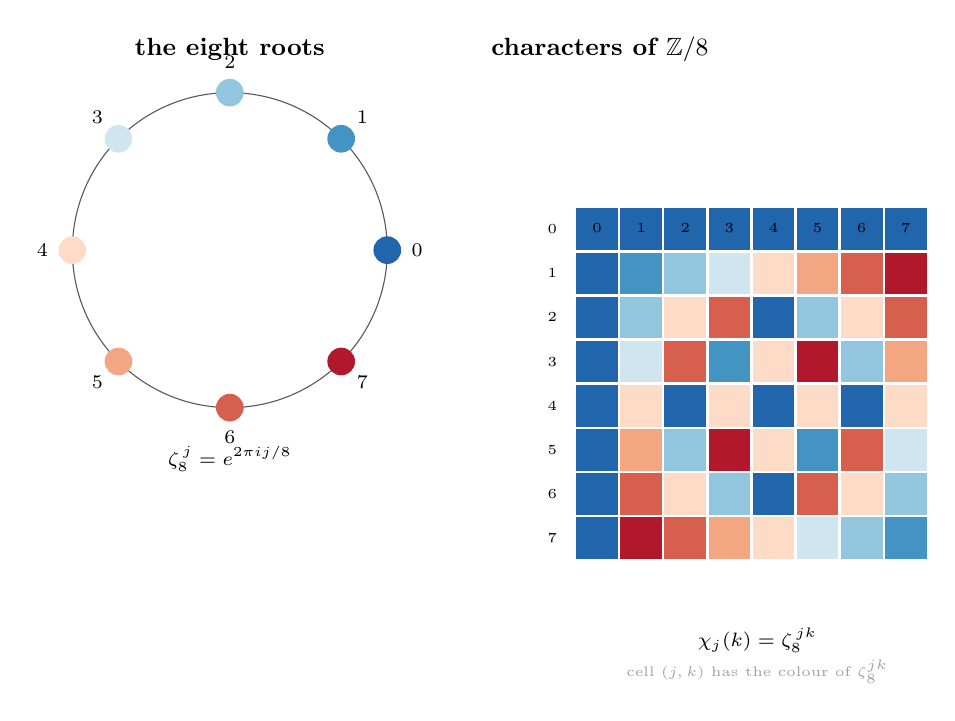
\begin{tikzpicture}
  % left: the eight roots
  \begin{scope}[xshift=-3.0cm]
    \draw[black!65] (0,0) circle (2.0);
    \foreach \j in {0,...,7} {%
      \pgfmathsetmacro{\ang}{45*\j}%
      \fill[c\j] (\ang:2.0) circle (5pt);%
      \node[font=\scriptsize] at (\ang:2.38) {\j};%
    }
    \node[font=\scriptsize] at (0,-2.65) {$\zeta_8^{\,j}=e^{2\pi i j/8}$};
  \end{scope}
  % right: the character matrix
  \begin{scope}[xshift=1.4cm]
    \foreach \j in {0,...,7} {%
      \foreach \k in {0,...,7} {%
        \pgfmathtruncatemacro{\cc}{mod(\j*\k,8)}%
        \fill[color=c\cc] ({\k*0.56},{-\j*0.56}) rectangle ++(0.53,0.53);%
      }%
      \node[font=\tiny,left] at (-0.12,{-\j*0.56+0.265}) {\j};%
    }
    \foreach \k in {0,...,7} {%
      \node[font=\tiny,above] at ({\k*0.56+0.265},0.10) {\k};%
    }
    \node[font=\scriptsize] at (2.3,-4.95) {$\chi_j(k)=\zeta_8^{\,jk}$};
    \node[font=\tiny,gray!75] at (2.3,-5.35) {cell $(j,k)$ has the colour of $\zeta_8^{jk}$};
  \end{scope}
  \node[font=\small\bfseries] at (1.7,2.55) {characters of $\mathbb Z/8$};
  \node[font=\small\bfseries] at (-3.0,2.55) {the eight roots};
\end{tikzpicture}
\end{document}
